%\VignetteIndexEntry{msiCompare--Class comparison for mass spectrometry imaging data}
%\VignetteKeyword{Bioinformatics, Proteomics, MassSpectrometry, ImagingMassSpectrometry}

\documentclass[a4paper]{article}\usepackage[]{graphicx}\usepackage[]{color}
%% maxwidth is the original width if it is less than linewidth
%% otherwise use linewidth (to make sure the graphics do not exceed the margin)
\makeatletter
\def\maxwidth{ %
  \ifdim\Gin@nat@width>\linewidth
    \linewidth
  \else
    \Gin@nat@width
  \fi
}
\makeatother

\definecolor{fgcolor}{rgb}{0.345, 0.345, 0.345}
\newcommand{\hlnum}[1]{\textcolor[rgb]{0.686,0.059,0.569}{#1}}%
\newcommand{\hlstr}[1]{\textcolor[rgb]{0.192,0.494,0.8}{#1}}%
\newcommand{\hlcom}[1]{\textcolor[rgb]{0.678,0.584,0.686}{\textit{#1}}}%
\newcommand{\hlopt}[1]{\textcolor[rgb]{0,0,0}{#1}}%
\newcommand{\hlstd}[1]{\textcolor[rgb]{0.345,0.345,0.345}{#1}}%
\newcommand{\hlkwa}[1]{\textcolor[rgb]{0.161,0.373,0.58}{\textbf{#1}}}%
\newcommand{\hlkwb}[1]{\textcolor[rgb]{0.69,0.353,0.396}{#1}}%
\newcommand{\hlkwc}[1]{\textcolor[rgb]{0.333,0.667,0.333}{#1}}%
\newcommand{\hlkwd}[1]{\textcolor[rgb]{0.737,0.353,0.396}{\textbf{#1}}}%
\let\hlipl\hlkwb

\usepackage{framed}
\makeatletter
\newenvironment{kframe}{%
 \def\at@end@of@kframe{}%
 \ifinner\ifhmode%
  \def\at@end@of@kframe{\end{minipage}}%
  \begin{minipage}{\columnwidth}%
 \fi\fi%
 \def\FrameCommand##1{\hskip\@totalleftmargin \hskip-\fboxsep
 \colorbox{shadecolor}{##1}\hskip-\fboxsep
     % There is no \\@totalrightmargin, so:
     \hskip-\linewidth \hskip-\@totalleftmargin \hskip\columnwidth}%
 \MakeFramed {\advance\hsize-\width
   \@totalleftmargin\z@ \linewidth\hsize
   \@setminipage}}%
 {\par\unskip\endMakeFramed%
 \at@end@of@kframe}
\makeatother

\definecolor{shadecolor}{rgb}{.97, .97, .97}
\definecolor{messagecolor}{rgb}{0, 0, 0}
\definecolor{warningcolor}{rgb}{1, 0, 1}
\definecolor{errorcolor}{rgb}{1, 0, 0}
\newenvironment{knitrout}{}{} % an empty environment to be redefined in TeX

\usepackage{alltt} 


\title{\texttt{msiCompare}: Class comparison for mass spectrometry imaging data}

\author{April J. Harry}
\IfFileExists{upquote.sty}{\usepackage{upquote}}{}
\begin{document}

\maketitle

\tableofcontents



\section{Introduction}
The \texttt{R} package \texttt{msiCompare} was built to provide access to the methods for class comparison in MSI described in this dissertation. \texttt{msiCompare} leverages the tools and data structures in the \texttt{Cardinal} package. When used in combination with \texttt{Cardinal}, it is possible to build a complete workflow from data preprocessing to statistical analysis all within \texttt{R}. In this chapter, we explore the main functionality of \texttt{msiCompare}.

The package is currently managed through a Github repository. The \texttt{devtools} package makes installation straightforward:

\begin{knitrout}
\definecolor{shadecolor}{rgb}{0.969, 0.969, 0.969}\color{fgcolor}\begin{kframe}
\begin{verbatim}
library(devtools)
install_github("ajharry/msiCompare")
\end{verbatim}
\end{kframe}
\end{knitrout}

Once installed, attach both the \texttt{msiCompare} and \texttt{Cardinal} packages.
\begin{knitrout}
\definecolor{shadecolor}{rgb}{0.969, 0.969, 0.969}\color{fgcolor}\begin{kframe}
\begin{verbatim}
library(msiCompare)
library(Cardinal)
\end{verbatim}
\end{kframe}
\end{knitrout}


\section{Simulating MS images}
We can simulate MSI data approximately according to Model \ref{model:prop}. For the n=1 situation, begin by defining two regions of interest which will represent the conditions to be compared. In the code below, condition 2 is defined as a square region in the center of a $30\times 30$ grid, while condition 1 is the bordering area.
\begin{knitrout}
\definecolor{shadecolor}{rgb}{0.969, 0.969, 0.969}\color{fgcolor}\begin{kframe}
\begin{verbatim}
conditions <- ifelse((expand.grid(x=1:30, y=1:30)$x %in% 
                        (1+floor(30/5)):(30-floor(30/5)) & 
                        expand.grid(x=1:30, y=1:30)$y %in% 
                        (1+floor(30/5)):(30-floor(30/5))), 2, 1)
\end{verbatim}
\end{kframe}
\end{knitrout}

The following function simulates the MS image. The algorithm works as follows:

\begin{enumerate}
\item Given a value for the spatial variance \texttt{tau2}, a \texttt{size1} $\times$ \texttt{size1} square grid of samples are drawn from the $properCAR(\rho, \texttt{tau2}, W)$ distribution, with $\rho = 0.9999$ (that is, nearly the $ICAR$ model). The neighborhood matrix $W$ is assumed to be binary with the 8-neighborhood structure. The samples are centered within each condition by default.
\item (\texttt{size1}$)^2$ independent samples are drawn from $\mathcal{N}$(mean = 0, var = \texttt{sig2}) to represent measurement error, and then added to the spatially correlated samples.
\item A value of \texttt{diff} is added to the simulated values for locations in condition 2 and zero to values for locations in condition 1.
\item This process is repeated \texttt{reps} times, with the sampled images returned as a \texttt{Cardinal} \texttt{MSImageSet} object.
\end{enumerate}

\begin{knitrout}
\definecolor{shadecolor}{rgb}{0.969, 0.969, 0.969}\color{fgcolor}\begin{kframe}
\begin{verbatim}
 s <- simSingle(
      reps = 3,
      diff = log2(1.5),
      tau2 = 0.1,
      sig2 = 0.1,
      seed = 8372,
      size1 = 30,
      pattern = conditions
      )
summary(s)
##        Length Class      Mode   
## simSet 1      MSImageSet S4     
## reps   1      -none-     numeric
## diff   1      -none-     numeric
## tau2   1      -none-     numeric
## sig2   1      -none-     numeric
## seed   1      -none-     numeric
## size1  1      -none-     numeric
## size2  1      -none-     numeric
\end{verbatim}
\end{kframe}
\end{knitrout}

Using \texttt{Cardinal} plotting tools, we can view the 3 simulated images.
\begin{knitrout}
\definecolor{shadecolor}{rgb}{0.969, 0.969, 0.969}\color{fgcolor}\begin{kframe}
\begin{verbatim}
image(s$simSet, feature = 1, layout = c(3,1))
image(s$simSet, feature = 2)
image(s$simSet, feature = 3)
\end{verbatim}
\end{kframe}

{\centering 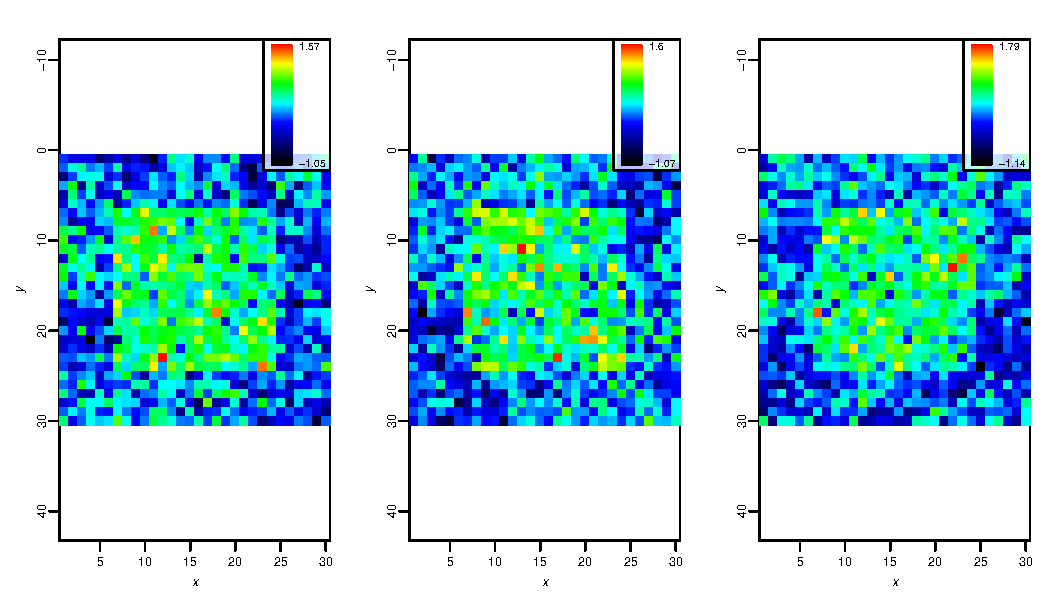
\includegraphics[width=\maxwidth]{figure/unnamed-chunk-5-1} 

}



\end{knitrout}

The specified conditions for each location are included in the \texttt{pixelData} of the \texttt{MSImageSet}.

\begin{knitrout}
\definecolor{shadecolor}{rgb}{0.969, 0.969, 0.969}\color{fgcolor}\begin{kframe}
\begin{verbatim}
head(pixelData(s$simSet))
## An object of class 'IAnnotatedDataFrame'
##   pixelNames: x = 1, y = 1 x = 2, y = 1 ... x = 6, y = 1 (6 total)
##   varLabels: x y sample diagnosis
##   varMetadata: labelType labelDescription
\end{verbatim}
\end{kframe}
\end{knitrout}

MSI datasets with $n>1$ are simulated similarly, with \texttt{diff} added to the simulated tissues for one of the conditions. Additionally, a value representing tissue-to-tissue biological variation drawn from $\mathcal{N}$(mean = 0, var = \texttt{sampleVar}) for each tissue and added to its simulated values.

\begin{knitrout}
\definecolor{shadecolor}{rgb}{0.969, 0.969, 0.969}\color{fgcolor}\begin{kframe}
\begin{verbatim}
 s_multi <- simMulti(
      sampleVar = 0.1,
      reps = 1,
      diff = log2(1.5),
      tau2 = 0.1,
      sig2 = 0.1,
      seed = 8372,
      size1 = 30,
      size2 = 30^2,
      numHealthy = 3,
      numDisease = 3)

image(s_multi$simSet, feature = 1, layout = c(3,2))
\end{verbatim}
\end{kframe}

{\centering 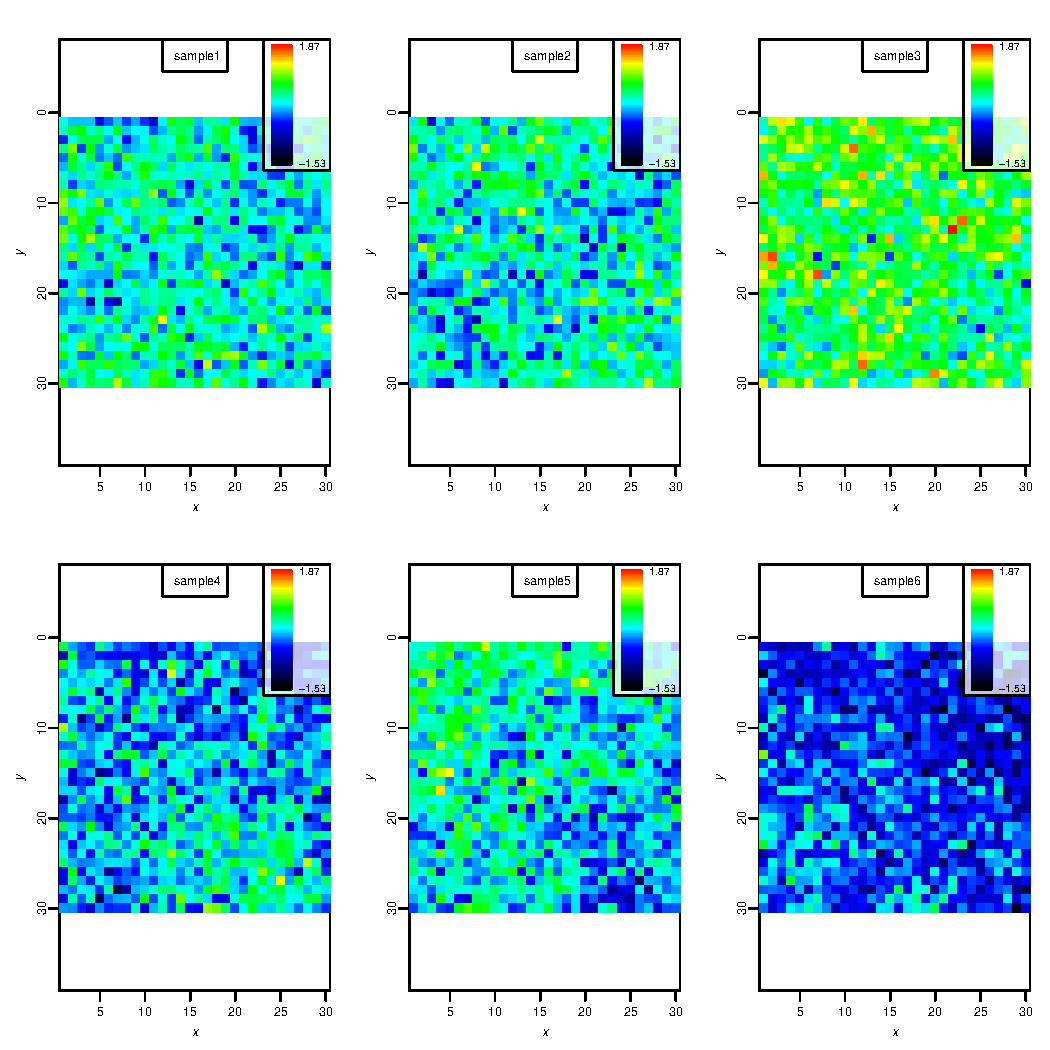
\includegraphics[width=\maxwidth]{figure/unnamed-chunk-7-1} 

}



\end{knitrout}

In addition to the condition at each pixel, the sample names are included in the \texttt{pixelData} of the \texttt{MSImageSet}.

\begin{knitrout}
\definecolor{shadecolor}{rgb}{0.969, 0.969, 0.969}\color{fgcolor}\begin{kframe}
\begin{verbatim}
head(pixelData(s_multi$simSet))
## An object of class 'IAnnotatedDataFrame'
##   pixelNames: x = 1, y = 1, sample = sample1 x = 2, y = 1, sample
##     = sample1 ... x = 6, y = 1, sample = sample1 (6 total)
##   varLabels: x y sample diagnosis
##   varMetadata: labelType labelDescription
\end{verbatim}
\end{kframe}
\end{knitrout}


\section{Statistical methods for class comparison}
\subsection{Hiearchical Bayesian Spatial Models}
The models described by Model \ref{model:prop} and the extensions in Equations \label{formula:spUnpaired} and \label{formula:Unpaired} are all available for use in the package. The models are fit using the Gibbs sampler MCMC algorithm detailed earlier in this chapter, with the hierarchical centring version of Section \ref{sec:HC} used for datasets with $n>1$.

The appropriate version of the model is chosen automatically based on the supplied arguments. The \texttt{conditionOfInterest} argument should be a vector representing the condition of each pixel, while the \texttt{techRep} vector must identify which tissue each pixel belongs to. The \texttt{bioRep} vector is optional; if the experiment has a subsampling or paired design then \texttt{bioRep} should identify which biological individual each pixel belongs to. These experimeal design arguments will often be columns in the \texttt{pixelData} of the \texttt{MSImageSet} object.

\begin{knitrout}
\definecolor{shadecolor}{rgb}{0.969, 0.969, 0.969}\color{fgcolor}\begin{kframe}
\begin{verbatim}
fitHBSM <- compareMSI(msset = s_multi$simSet,
           conditionOfInterest = s_multi$simSet$diagnosis,
           techRep = s_multi$simSet$sample,
           bioRep = NULL,
           feature = 1,
           nsim = 5000, burnin=2500,
           trace = T, dropZeros = F)
\end{verbatim}
\end{kframe}
\end{knitrout}

From the model fit we can access point estimates of the parameters of interest, such as the posterior probability of differential abundance.
\begin{knitrout}
\definecolor{shadecolor}{rgb}{0.969, 0.969, 0.969}\color{fgcolor}\begin{kframe}
\begin{verbatim}
fitHBSM$Feature1$gamma
## [1] 0.03278689
\end{verbatim}
\end{kframe}
\end{knitrout}

We have also implemented the BFDR thresholding procedure (Chapter \ref{chap:proposed} and {Ventrucci2011}) to adjust for multiple comparisons.
\begin{knitrout}
\definecolor{shadecolor}{rgb}{0.969, 0.969, 0.969}\color{fgcolor}\begin{kframe}
\begin{verbatim}
postProbs <- runif(100) #simulating 100 posterior probabilities
bfdr <- BFDRdecision(postProbs, alpha = 0.05)
table(bfdr)
## bfdr
## FALSE  TRUE 
##    91     9
\end{verbatim}
\end{kframe}
\end{knitrout}

If the \texttt{trace} argument in \texttt{compareMSI} is set to \texttt{TRUE}, then the trace of the MCMC samples is returned.

\begin{knitrout}
\definecolor{shadecolor}{rgb}{0.969, 0.969, 0.969}\color{fgcolor}\begin{kframe}
\begin{verbatim}
plot(fitHBSM$Feature1$trace[,1], 
     density = F, main = "Trace of baseline effect")
\end{verbatim}
\end{kframe}

{\centering 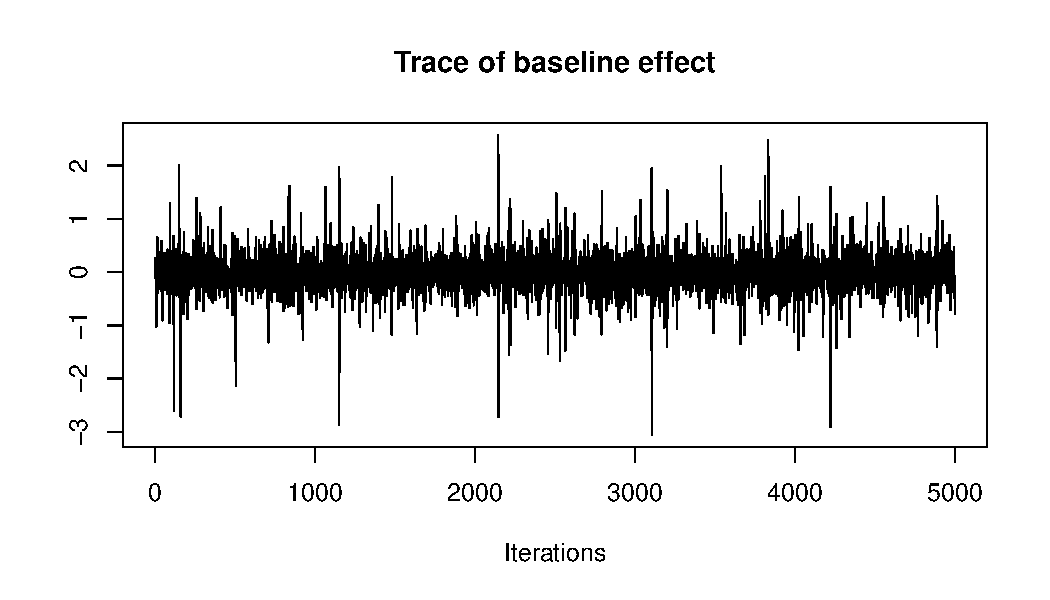
\includegraphics[width=\maxwidth]{figure/unnamed-chunk-12-1} 

}



\end{knitrout}

\subsection{Spatial modeling for MSI, as described in Cassese, et al}
The spatial model proposed in {Cassese2016} is also available in the package. The code is based on the implementation in the supplementary information for {Cassese2016}, with a wrapper to streamline its use with \texttt{Cardinal} objects.

\begin{knitrout}
\definecolor{shadecolor}{rgb}{0.969, 0.969, 0.969}\color{fgcolor}\begin{kframe}
\begin{verbatim}
fit_spautolm <- cass(msset = s$simSet, 
                     roiFactor = factor(s$simSet$diagnosis),
                     logscale = F, thresholds = 1:5)
\end{verbatim}
\end{kframe}
\end{knitrout}
\begin{knitrout}
\definecolor{shadecolor}{rgb}{0.969, 0.969, 0.969}\color{fgcolor}\begin{kframe}
\begin{verbatim}
fit_spautolm$results$CAR_AIC_min_pvalues
## [1] 0 0 0
\end{verbatim}
\end{kframe}
\end{knitrout}


\subsection{ANOVA}
ANOVA methods (Models \ref{model:locANOVA} and \ref{model:locANOVA}) are available natively in \texttt{R}, but we show them here for completeness:
\begin{knitrout}
\definecolor{shadecolor}{rgb}{0.969, 0.969, 0.969}\color{fgcolor}\begin{kframe}
\begin{verbatim}
##### Location-wise ANOVA #####
intensities <- c(spectra(s_multi$simSet)[1,])
conditions <- s_multi$simSet$diagnosis

# summary of model fit
coef(summary(lm(intensities~conditions))) 
##                      Estimate  Std. Error   t value      Pr(>|t|)
## (Intercept)       -0.03924918 0.008125954 -4.830102  1.402342e-06
## conditionsHealthy  0.44145207 0.011491835 38.414412 1.242852e-285
\end{verbatim}
\end{kframe}
\end{knitrout}


\begin{knitrout}
\definecolor{shadecolor}{rgb}{0.969, 0.969, 0.969}\color{fgcolor}\begin{kframe}
\begin{verbatim}
##### Tissue-wise ANOVA #####
sampNames <- sampleNames(s_multi$simSet)
samps <- s_multi$simSet$sample 

# get tissue averages
averages <- sapply(sampNames, 
                   function(s) mean(intensities[samps== s]))

#condition for each tissue
conditions <- factor(c("Healthy","Healthy","Healthy",
                       "Disease","Disease","Disease"))

#summary of model fit
coef(summary(lm(averages ~ conditions))) 
##                      Estimate Std. Error   t value  Pr(>|t|)
## (Intercept)       -0.03924918  0.1469225 -0.267142 0.8025676
## conditionsHealthy  0.44145207  0.2077799  2.124614 0.1008170
\end{verbatim}
\end{kframe}
\end{knitrout}

\end{document}

